\documentclass[10pt]{beamer}

\usetheme{metropolis}
\usepackage{appendixnumberbeamer}

\usepackage{booktabs}
\usepackage[scale=2]{ccicons}

\usepackage{pgfplots}
\usepgfplotslibrary{dateplot}

\usepackage{xspace}

\usepackage{tikz}
	\usetikzlibrary{shapes.geometric, arrows, positioning}
	\tikzstyle{startstop} = [rectangle, rounded corners, minimum width=3cm, minimum 		height=1cm,text centered, draw=black, fill=red!30]
	\tikzstyle{io} = [trapezium, trapezium left angle=70, trapezium right angle=110, minimum width=3cm, minimum height=1cm, text centered, draw=black, fill=blue!30]
	\tikzstyle{process} = [rectangle, minimum width=3cm, minimum height=1cm, text centered, draw=black, fill=orange!30]
\tikzstyle{decision} = [diamond, minimum width=3cm, minimum height=1cm, text centered, draw=black, fill=green!30]
\tikzstyle{arrow} = [thick,->,>=stealth]
\tikzstyle{arrow} = [thick,->,>=stealth]
%\usepackage{listings}
\usepackage{minted}

\usepackage{bm}%................................. Bold math symbols (after fonts)

\setbeamercolor{normal text}{bg=white}





\title{EML4930/EML6934: Lecture 13}
\subtitle{Pandas - Python Data Analysis Library}
\date{November 30, 2017}
%\author{CJ}
\author{Charles Jekel}
%\titlegraphic{\includegraphics{images/avatarCropped.png}\vspace{58cm}}
%\institute{1. University of Florida\\ 2. Stellenbosch University, South Africa}

% \titlegraphic{\hfill\includegraphics[height=1.5cm]{logo.pdf}}

\begin{document}

\maketitle

\begin{frame}{Format of final}
Sample Questions posted online.

Final will be 21 questions, were 20 questions are graded. (So there will be one bonus question.) Questions will be similar the quiz questions.

\textbf{Monday December 11, 8:30 am - 9:30 am - MAEA 303}
\end{frame}

\begin{frame}{Questions you will definitely be asked}
\begin{itemize}
\item Differences between Python 2 and Python 3
\item Anything about the Python syntax
\item Loops in Python
\item Functions in Python
\item NumPy operations (arrays and multiplication) 
\item Matplotlib plotting
\item Concept questions related to your understanding of Python things
\item How to update libraries via command
\item How to open a file in Python
\end{itemize}
\end{frame}

\begin{frame}{Course Evaluations are important}
I currently only have a 32\% course evaluation response rate. The last date to provide a course evaluation is December 8th. 

Do not wait until the last minute!

Please go to \url{https://evaluations.ufl.edu} right now and fill out an evaluation if you haven't already.  

Evaluations are the only official means to critique this course and myself.
\end{frame}

\begin{frame}{Pandas - Python Data Analysis Library}
pandas is an open source, BSD-licensed library providing high-performance, easy-to-use data structures and data analysis tools for the Python programming language.

\url{https://pandas.pydata.org/}

What does pandas solve?
  \begin{quote}
    Python has long been great for data munging and preparation, but less so for data analysis and modeling. pandas helps fill this gap, enabling you to carry out your entire data analysis workflow in Python without having to switch to a more domain specific language like R.
\end{quote}

\end{frame}

\begin{frame}{Useful resources on learning pandas}
Python for Data Analysis, 2nd Edition Data Wrangling with Pandas, NumPy, and IPython, Wes McKinney \url{http://shop.oreilly.com/product/0636920050896.do}

\url{https://github.com/wesm/pydata-book}

Python Data Science Handbook, Essential Tools for Working with Data, Jake VanderPlas \url{http://shop.oreilly.com/product/0636920034919.do}

\url{https://github.com/jakevdp/PythonDataScienceHandbook}

\url{https://github.com/jvns/pandas-cookbook}
\end{frame}

\begin{frame}{pandas consists of the following elements}

\begin{itemize}
\item A set of labeled array data structures, the primary of which are Series and DataFrame
\item Index objects enabling both simple axis indexing and multi-level / hierarchical axis indexing
\item An integrated group by engine for aggregating and transforming data sets
\item Date range generation (date\_range) and custom date offsets enabling the implementation of customized frequencies
\item Input/Output tools: loading tabular data from flat files (CSV, delimited, Excel 2003), and saving and loading pandas objects from the fast and efficient PyTables/HDF5 format.
\item Memory-efficient "sparse" versions of the standard data structures for storing data that is mostly missing or mostly constant (some fixed value)
\item Moving window statistics (rolling mean, rolling standard deviation, etc.)
\end{itemize}
\end{frame}

\begin{frame}[fragile]{pandas import}
\begin{minted}
{python}
import pandas as pd
# pd is the standard pandas alias
\end{minted}
\end{frame}

\begin{frame}[fragile]{pandas objects}
\begin{table}
\begin{tabular}{lc}
\textbf{Object} & \textbf{Description} \\
\hline
pd.Series & One-dimensional ndarray with axis labels. \\
pd.DataFrame & Two-dimensional size-mutable, row and column data. \\
pd.Index & Immutable ndarray for sorting axis labels. 
\end{tabular}
\end{table}
\end{frame}

\begin{frame}[fragile]{pandas Series}
\begin{minted}
{python}
# create arbitrary series from list
data = pd.Series([0.2, 0.4, 0.6, 0.27])

print(data)

# The Series will contain attributes named values and index
# data.values contains the numpy array
print(data.values)

# data.index contains the pandas Index object for the Series
print(data.index)

# you can slice pandas Series just like a numpy array
print(data[1])
print(data[0:2])

# so why Series over numpy array?
\end{minted}
\end{frame}

\begin{frame}[fragile]{Explicit index definition for Series}
\begin{minted}
{python}
# create arbitrary series from list
data = pd.Series([0.2, 0.4, 0.6, 0.27], index=['a','b','c','d'])

# data.index will now contain the letters a-d
print(data.index)

# you can still slice pandas Series just like a numpy array
print(data[0:2])

# or you can access the data with the index specific keys
print(data['a'])
print(data['b'])
# so this is kind of like a specialized dictionary... 
# Dictionary: arbitrary keys -> set of arbitrary values
# Series: typed keys -> set of typed value
# Essentially Series are more efficient than Dictionaries
\end{minted}
\end{frame}

\begin{frame}[fragile]{Building a series from dictionary}
\begin{minted}
{python}
my_dict = {'Germany': 'sauerkraut', 'Spain': 'paella',
 'Italy': 'pizza', 'USA': 'Hamburger'}
my_series = pd.Series(my_dict)

# unlike dictionaries you can access a Series with slicing
print(my_series['Spain':'USA'])
\end{minted}
\end{frame}

\begin{frame}{So about this immutable Index object...}
\begin{itemize}
\item thought of as immutable array and ordered multiset
\item immutable = cannot be modified
\item combination of Python set and 1D numpy array
\end{itemize}
\end{frame}

\begin{frame}[fragile]{Creating an Index object}
\begin{minted}
{python}
# create arbitrary Index
indA = pd.Index([1, 3, 5, 7, 9])
indB = pd.Index([2, 3, 5, 7, 11])

# You can access an index like you would a numpy array
print(indA[1:3])

# You can also use Pythons builtin set notation
print(indA & indB) # intersection
print(indA | indB) # union
print(indA ^ indB) # symmetric difference

\end{minted}
\end{frame}

\begin{frame}{What is a pandas DataFrame?}
DataFrame is a 2-dimensional labeled data structure with columns of potentially different types. You can think of it like a spreadsheet or SQL table, or a dict of Series objects. It is generally the most commonly used pandas object. Like Series, DataFrame accepts many different kinds of input:
\begin{itemize}
\item Dict of 1D ndarrays, lists, dicts, or Series
\item 2-D numpy.ndarray
\item Structured or record ndarray
\item A Series
\item Another DataFrame
\end{itemize}
Along with the data, you can optionally pass index (row labels) and columns (column labels) arguments. 

and more: \url{https://pandas.pydata.org/pandas-docs/stable/dsintro.html}
\end{frame}

\begin{frame}[fragile]{Creating a DataFrame}
\begin{minted}
{python}
population_dict = {'California': 38332521,'Texas': 26448193,
 'New York': 19651127, 'Florida': 19552860,
 'Illinois': 12882135} 
area_dict = {'California': 423967, 'Texas': 695662, 
'New York': 141297, 'Florida': 170312, 'Illinois': 149995}
# let's first create a series from these dictionaries
population = pd.Series(population_dict)
area = pd.Series(area_dict)

# create a DataFrame from these two Series
states = pd.DataFrame({'population': population, 'area': area})
print(states)

# DataFrame will have index and values attributes
print(states.index) # pandas Index object
print(states.values) # Two dimensional numpy array
\end{minted}
\end{frame}

\begin{frame}[fragile]{Access the 'rows' and 'columns'}
\begin{minted}
{python}
# you can think of the index as the rows of the table
print(states.index)

# to access a row you need to use .loc
print(states.loc['Florida'])

# and can find the columns by
print(states.columns)

# you can access the area column by
print(states['area'])

\end{minted}
\end{frame}

\begin{frame}{Ways to create DataFrame}
\begin{itemize}
\item From Series object
\item From list of dictionaries
\item From dictionary of Series objects
\item From two-dimensional numpy array
\item From numpy structured array
\end{itemize}
\end{frame}

\begin{frame}[fragile]{Examples of creating DataFrames}
\begin{minted}
{python}
# DataFrames will automatically fill missing values with NaNs
# integers are automatically used as the index (like Series)
in : pd.DataFrame([{'a': 1, 'b': 2}, {'b': 3, 'c': 4}])
out:     
   a    b    c
0  1.0  2  NaN
1  NaN  3  4.0

# You can feed a 2D numpy array, and manually pass the 
# columns and index (rows) names
in : pd.DataFrame(np.random.rand(3, 2),columns=['foo', 'bar'],
                  index=['a', 'b', 'c'])
out:         
   foo       bar
a  0.610023  0.239564
b  0.141317  0.315237
c  0.221186  0.316919
\end{minted}
\end{frame}

\begin{frame}[fragile]{Pandas uses int64 and float64 by default!}
NumPy floats will be float64 by default, however NumPy integers will be int32 if small... 
\begin{minted}
{python}
a = np.array((1,2,12,121))
print(a.dtype) # this will print int32!

b = np.array((2165156165151,15165,1561121261))
print(b.type) # this will print int64

# however looking at our DataFrame
print(states.dtypes)
# we'll see int64
\end{minted}
\end{frame}



\begin{frame}[fragile]{DataFrame loc vs iloc}
Recall how I said you can access the row of a DataFrame with loc?
\begin{minted}
{python}
mydf = pd.DataFrame(np.random.rand(3, 2),columns=['foo', 'bar'],
                  index=['a', 'b', 'c'])

# Use .loc to access the explicit index
print(mydf.loc['b'])

# Use .iloc to access the implicit Python-style index 
print(mydf.iloc[1])
\end{minted}
\end{frame}

\begin{frame}[fragile]{Creating a new column in DataFrame}
\begin{minted}
{python}
# recall our state data
states = pd.DataFrame({'population': population, 'area': area})

# we can make a new population density column by accessing the
# DataFrame like a dictionary
states['density'] = states['population']/ states['area']

print(states)

# NOTE:
# Even with Python 2 density will automatically be float64 
# this happens by default in pandas
\end{minted}
\end{frame}

\begin{frame}[fragile]{More ways to manipulate DataFrames}
\begin{minted}
{python}
# swapping rows for columns using .T
print( states.T ) 

# accessing a row of the numpy array
print( states.values[0] )

# accessing the first three rows, and first two columns
print( states.iloc[:3, :2] )
\end{minted}
\end{frame}

\begin{frame}[fragile]{Accessing data frames with masking}
\begin{minted}
{python}
# you can select just the states that have a density > 100
in : states.loc[ states['density'] > 100 ]  
out: 
            area  population     density
Florida   170312    19552860  114.806121
New York  141297    19651127  139.076746

# masking and selection of columns
in : states.loc[ states['density'] > 100,['area', 'population']]  
out: 
            area  population
Florida   170312    19552860
New York  141297    19651127
\end{minted}
\end{frame}

\begin{frame}[fragile]{How to add a row to a DataFrame}
\begin{minted}
{python}
# let's say we have the following list which corresponds to the area,
# population, and density of Colorado 
co_data = [269601, 5540545, 20.5509]

# We'll create a new Series from this list using the columns as the index
# and giving a name to the series as Colorado 
new = pd.Series(co_data, index=states.columns, name='Colorado')

# you need to set states = states.append! as states.append won't save the
# DataFrame!
states = states.append(new)

# you'll you a new Row named Colorado
print( states ) 
\end{minted}
\end{frame}

\begin{frame}[fragile]{How to remove duplicates from a DataFrame}
\begin{minted}
{python}
                area  population     density
California  423967.0  38332521.0   90.413926
Florida     170312.0  19552860.0  114.806121
Illinois    149995.0  12882135.0   85.883763
New York    141297.0  19651127.0  139.076746
Texas       695662.0  26448193.0   38.018740
Colorado    269601.0   5540545.0   20.550900
Colorado    269601.0   5540545.0   20.550900

# This is an easy fix! just run drop_duplicates()
states = states.drop_duplicates()

# This will remove the duplicate Colorado row!
\end{minted}
\end{frame}

\begin{frame}[fragile]{How to add a column to a DataFrame}
\begin{minted}
{python}
# let's add the electoral votes to the DataFrame
# First let's create a dictionary of what we want to add
votes = {'California': 55, 'Colorado': 9, 'Florida': 29,
 'Illinois': 20, 'New York': 29, 'Texas': 38}
# now let's turn the dictionary into a pd series
votes = pd.Series(votes)
# Now we'll use the assign function to add a column named
# electoral to the DataFrame
states = states.assign(electoral=votes)

# we now have:
                area  population     density  electoral
California  423967.0  38332521.0   90.413926         55
Florida     170312.0  19552860.0  114.806121         29
Illinois    149995.0  12882135.0   85.883763         20
New York    141297.0  19651127.0  139.076746         29
Texas       695662.0  26448193.0   38.018740         38
Colorado    269601.0   5540545.0   20.550900          9
\end{minted}
\end{frame}

\begin{frame}[fragile]{Other useful DataFrame functions}
\begin{table}
\begin{tabular}{ll}
\textbf{Function} & \textbf{Description} \\
\hline
head & Returns the first $n$ rows (default 5) \\
tail & Returns the last $n$ rows (default 5)\\
describe & Statistic summary of the data\\
group\_by & Group by a series or column \\
plot & DataFrame plotting method \\
value\_counts & Count the number of occurrences in a series\\
replace & replace(oldvalue, newvalue) in a DataFrame \\
dropna & remove all rows from DataFrame that contain a NaN value\\
\end{tabular}
\end{table}
\end{frame}

\begin{frame}{So where will I most likely use DataFrames?}
\begin{itemize}
\item If you have spreadsheet data (csv, xls, ...)
\item SQL data
\item Various other databases... 
\end{itemize}
\textbf{To read and write CSV files.}
\end{frame}

\begin{frame}[fragile]{How to open a CSV file as DataFrame}
\url{https://pandas.pydata.org/pandas-docs/stable/generated/pandas.read_csv.html}
This has more options than any other Python function I've ever seen...
\begin{minted}
{python}
pd.read_csv(filepath_or_buffer, sep=', ', delimiter=None, 
header='infer', names=None, index_col=None, usecols=None,
 squeeze=False, prefix=None, mangle_dupe_cols=True, 
 dtype=None, engine=None, converters=None, true_values=None,
 false_values=None, skipinitialspace=False, skiprows=None,
 nrows=None, na_values=None, keep_default_na=True, 
 na_filter=True, verbose=False, skip_blank_lines=True,
 parse_dates=False, infer_datetime_format=False, 
 keep_date_col=False, date_parser=None, dayfirst=False,
 iterator=False, chunksize=None, compression='infer', 
 thousands=None, decimal=b'.', lineterminator=None, 
 quotechar='"', quoting=0, escapechar=None, comment=None,
 encoding=None, dialect=None, tupleize_cols=None, 
 error_bad_lines=True, warn_bad_lines=True, skipfooter=0, 
 skip_footer=0, doublequote=True, delim_whitespace=False, 
 as_recarray=None, compact_ints=None, use_unsigned=None, 
 low_memory=True, buffer_lines=None, memory_map=False, 
 float_precision=None)
\end{minted}
\end{frame}

\begin{frame}[fragile]{Basic pd.read\_csv}
\begin{minted}
{python}
# TSLA is the stock data for Tesla
# create a DataFrame named tsla from TSLA.csv
tsla = pd.read_csv('TSLA.csv')

# pandas will automatically create an Index
print(tsla.head())


         Date       Open   High        Low      Close  Adj Close    Volume
0  2010-06-29  19.000000  25.00  17.540001  23.889999  23.889999  18766300
1  2010-06-30  25.790001  30.42  23.299999  23.830000  23.830000  17187100
2  2010-07-01  25.000000  25.92  20.270000  21.959999  21.959999   8218800
3  2010-07-02  23.000000  23.10  18.709999  19.200001  19.200001   5139800
4  2010-07-06  20.000000  20.00  15.830000  16.110001  16.110001   6866900
\end{minted}
\end{frame}

\begin{frame}[fragile]{You can explicitly load the csv stating the index column}
\begin{minted}
{python}
# create a DataFrame named tsla from TSLA.csv
# let's use Date as the index of the DataFrame
tsla = pd.read_csv('TSLA.csv', index_col='Date')

print(tsla.head())


                 Open   High        Low      Close  Adj Close    Volume
Date                                                                   
2010-06-29  19.000000  25.00  17.540001  23.889999  23.889999  18766300
2010-06-30  25.790001  30.42  23.299999  23.830000  23.830000  17187100
2010-07-01  25.000000  25.92  20.270000  21.959999  21.959999   8218800
2010-07-02  23.000000  23.10  18.709999  19.200001  19.200001   5139800
2010-07-06  20.000000  20.00  15.830000  16.110001  16.110001   6866900
\end{minted}
\end{frame}

\begin{frame}[fragile]{Sometimes null or na strings will mess up the data type}
\begin{minted}
{python}
# so let's say our csv file has a bunch of 'null' strings 
# that are messing up our analysis...
             Open   High        Low      Close  Adj Close    Volume
Date                                                               
2010-06-29   null  25.00  17.540001  23.889999  23.889999  18766300
2010-06-30  25.79  30.42  23.299999  23.830000  23.830000  17187100

# The Open column will have an Object data type because it has
# strings and floats, one way to get rid of this is to load the csv using
# this will setup all 'null' strings to be a np.NaN (a float)
tsla =pd.read_csv('TSLA.csv',index_col='Date',na_values='null')

print(tsla.head())
             Open   High        Low      Close  Adj Close    Volume
Date                                                               
2010-06-29    NaN  25.00  17.540001  23.889999  23.889999  18766300
2010-06-30  25.79  30.42  23.299999  23.830000  23.830000  17187100
2010-07-01     25  25.92  20.270000  21.959999  21.959999   8218800
2010-07-02     23  23.10  18.709999  19.200001  19.200001   5139800
2010-07-06     20  20.00  15.830000  16.110001  16.110001   6866900
\end{minted}
\end{frame}

\begin{frame}[fragile]{Saving the csv file}
\url{https://pandas.pydata.org/pandas-docs/stable/generated/pandas.DataFrame.to_csv.html}
\begin{minted}
{python}
# so let's create a new column based on the other columns
tsla['avg'] = .25*(tsla['Open'] + tsla['High'] \ 
              + tsla['Low'] + tsla['Close'])
              
# we can create a new csv by running
tsla.to_csv('my_new.csv')
\end{minted}
\end{frame}

\begin{frame}[fragile]{Plotting data with from a DataFrame}
\begin{minted}
{python}
import matplotlib.pyplot as plt
import seaborn # for styling
seaborn.set()  # for styling

tsla.['Close'].plot()
\end{minted}
\begin{figure}
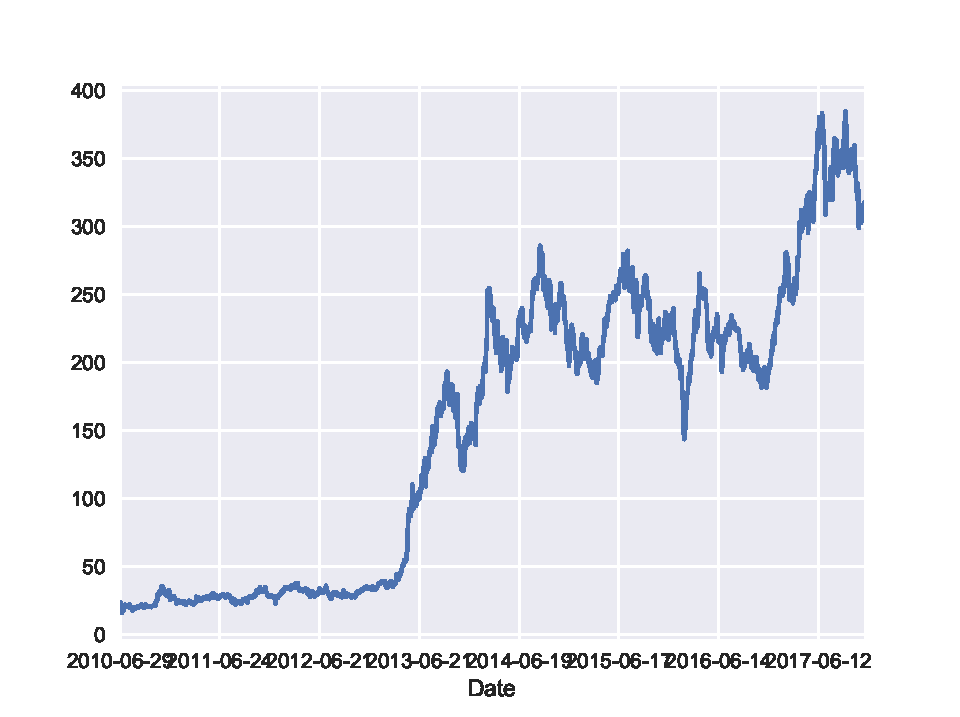
\includegraphics[width=0.7\textwidth]{figs/1.pdf}
\end{figure}
\end{frame}

\begin{frame}[fragile]{Pandas handles Time Series data really well}
\begin{minted}
{python}
# plot just the close price for 2016
tsla['Close'].loc['2016':'2017'].plot()
\end{minted}
\begin{figure}
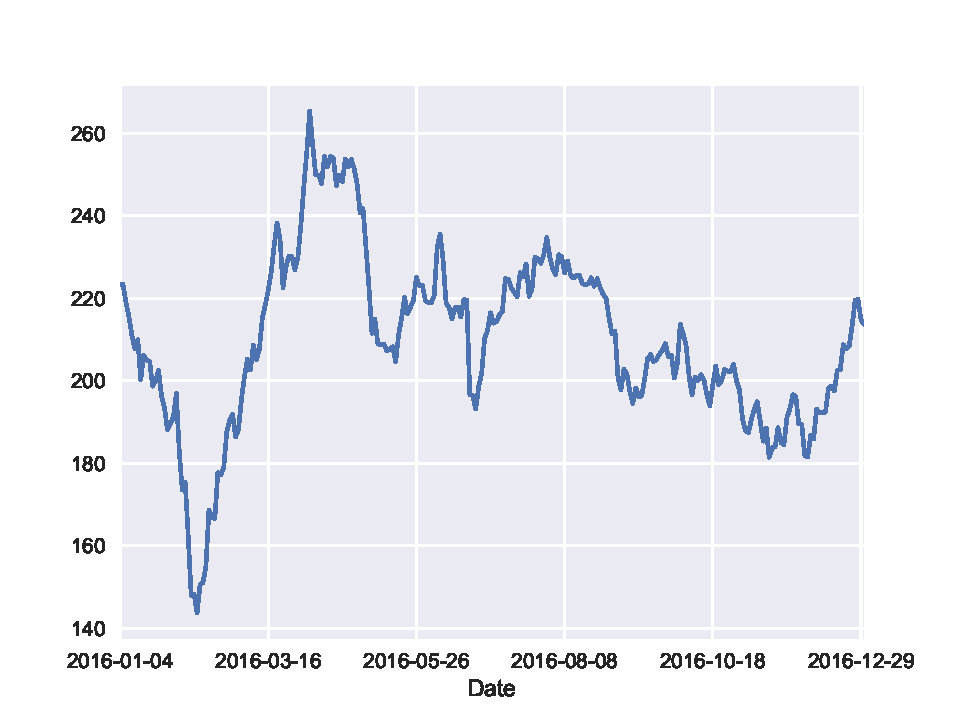
\includegraphics[width=0.7\textwidth]{figs/2.pdf}
\end{figure}
\end{frame}

\begin{frame}[fragile]{Creating date-time sequences with pandas}
\begin{minted}
{python}
in : pd.date_range('2017-01-03', '2017-01-10')
out: DatetimeIndex(['2017-01-03', '2017-01-04', '2017-01-05',
 '2017-01-06', '2017-01-07', '2017-01-08', '2017-01-09', 
 '2017-01-10'],dtype='datetime64[ns]', freq='D')
              
in : pd.date_range('2017-07-03', periods=8)
out: DatetimeIndex(['2017-07-03', '2017-07-04', '2017-07-05',
 '2017-07-06','2017-07-07', '2017-07-08', '2017-07-09', 
 '2017-07-10'], dtype='datetime64[ns]', freq='D')
              
in : pd.date_range('1999-07-03', periods=4, freq='H')
out: 
DatetimeIndex(['1999-07-03 00:00:00', '1999-07-03 01:00:00',
               '1999-07-03 02:00:00', '1999-07-03 03:00:00'],
              dtype='datetime64[ns]', freq='H')
\end{minted}
\end{frame}

\begin{frame}[fragile]{Creating date-time sequences with pandas}
\begin{minted}
{python}
in : pd.period_range('1943-03', periods=8, freq='M')
out: PeriodIndex(['1943-03', '1943-04', '1943-05', '1943-06', 
     '1943-07', '1943-08', '1943-09', '1943-10'], 
     dtype='period[M]', freq='M')
 
in : pd.timedelta_range(0, periods=10, freq='H')
out: TimedeltaIndex(['00:00:00', '01:00:00', '02:00:00', 
    '03:00:00', '04:00:00', '05:00:00', '06:00:00', 
    '07:00:00', '08:00:00', '09:00:00'],
     dtype='timedelta64[ns]', freq='H')

\end{minted}
\end{frame}

\begin{frame}{So Why use Pandas}
\begin{itemize}
\item Useful function for working with databases
\item DataFrames can be manipulated easier than lists
\item For exporting and importing CSV files in Python
\item Working with time series data
\end{itemize}
\end{frame}

\begin{frame}{Thanks for taking my class!}
Hopefully you've learned something about Python.
\end{frame}
%\begin{frame}{More with Scikit-Learn}
%\begin{itemize}
%\item Saving Python objects with Pickle
%\item Saving Scikit-Learn models with joblib
%\item Cross Validation
%\item Neural Network Example 
%\end{itemize}
%\end{frame}
%
%\begin{frame}[fragile]{Saving Python objects with Pickle}
%\begin{minted}
%{python}
%# This code fits a support vector classifier to the iris dataset
%from sklearn import svm
%from sklearn import datasets
%clf = svm.SVC()
%iris = datasets.load_iris()
%X, y = iris.data, iris.target
%clf.fit(X, y)  
%
%# we can use Python's pickle to save the clf object
%# pickle writes an object's memory state
%import pickle
%# save the clf object to 'my_svc_clf.p'
%pickle.dump( clf, open('my_svc_clf.p', 'wb'))
%
%# load clf object using
%clf = pickle.load( open('my_svc_clf.p', 'rb'))
%
%\end{minted}
%\end{frame}
%
%\begin{frame}[fragile]{You should use cPickle in Python 2}
%In Python 2 you should use cPickle which is up to 1000 time faster than pickle. Python 3 automatically uses cPickle (if available). 
%\begin{minted}
%{python}
%# importing from cPickle in Python 2
%import cPickle as pickle
%\end{minted}
%
%However this import will break Python 3 code
%\end{frame}
%
%\begin{frame}[fragile]{We can use Try: Except: to write a Python X}
%\begin{minted}
%{python}
%# this code will import pickle on both Python 2 and Python 3
%try: 
%    # first let's try importing 
%    import cPickle as pickle
%    # if this returns an error, it isn't shown
%    # rather the code from except: is run
%except:
%    # this only runs if the try code had an error
%    import pickle
%\end{minted}
%\end{frame}
%
%\begin{frame}{Summary of pickle}
%\begin{itemize}
%\item Pickle objects can be hacked
%\item Don't load a pickled object if you can't trust the source
%\item Malicous code can be executed when loading a Pickled objected
%\item You can use Pickle to save any Python object
%\item If you use Python 2, you should use cPickle as it's 1000 times faster!
%\end{itemize}
%\end{frame}
%
%\begin{frame}[fragile]{Saving Scikit-Learn models with joblib}
%Scikit-Learn recommends using joblib over pickle to save models as it's more efficient with 
%large numpy arrays. 
%\begin{minted}
%{python}
%from sklearn import svm
%from sklearn import datasets
%clf = svm.SVC()
%iris = datasets.load_iris()
%X, y = iris.data, iris.target
%clf.fit(X, y) 
%
%from sklearn.externals import joblib
%# save the clf object using
%joblib.dump(clf, 'filename.pkl')
%
%# load the .pkl file to clf using
%clf = joblib.load('filename.pkl') 
%\end{minted}
%\end{frame}
%
%\begin{frame}{Why do we want to be able to save and open models?}
%\textbf{because some models may take a long time to train as we want to used a trained model to predict for the future}
%\end{frame}
%
%\begin{frame}{Scikit-learn has lots of models}
%\begin{itemize}
%\item Naive Bayes
%\item Linear regression
%\item Support Vector Machines
%\item Decision Trees and Random Forests
%\item Gaussian process prediction
%\end{itemize}
%so which model do we use?
%\end{frame}
%
%\begin{frame}{Cross Validation for model validation}
%\begin{itemize}
%\item Cross Validation (CV) is a tool for model selection on the principle that data collection is expensive (we can't afford to obtain more data points)
%\item Used to estimate how accurately a predictive model will perform in practice
%\item There are various CV variations, I'm going to focus on k-fold CV
%\end{itemize}
%\end{frame}
%
%\begin{frame}{K-fold Cross Validation}
%\begin{enumerate}
%\item Partition the data into $k$ equal sized sets of samples 
%\item Train the model on $k-1$ sample sets, validate the model (score) on the single remaining set
%\item Iterate $k$ times
%\item Final K-fold CV metric is the average score from each iteration
%\end{enumerate}
%\end{frame}
%
%\begin{frame}{4-fold CV visualized}
%\begin{figure}
%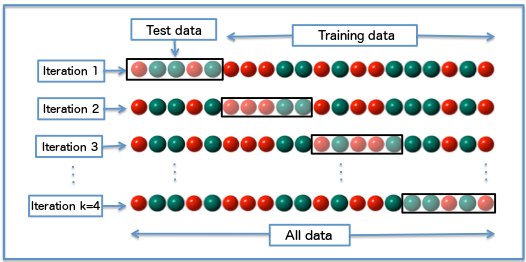
\includegraphics[width=1.0\textwidth]{figs/cv.jpg}
%\caption{Visualization of a 4-fold CV. CC BY-SA 3.0 author Fabian Fl\"ock }
%\end{figure}
%\end{frame}
%
%\begin{frame}{K-fold CV tips}
%\begin{itemize}
%\item In practice $k$ can be anywhere between 5-20
%\item There is no best $k$
%\item 10-fold CV is really common
%\item everyone developes their own preference
%\item Use for model validation
%\item Use to approximate the accuracy of the model
%\end{itemize}
%\end{frame}
%
%\begin{frame}[fragile]{Scikit-learn includes a KFold CV iterator}
%Use KFold as a cross validation iterator.
%\begin{minted}
%{python}
%from sklearn import svm
%from sklearn import datasets
%clf = svm.SVC()
%iris = datasets.load_iris()
%X, y = iris.data, iris.target
%
%# import the cross validation iterator
%from sklearn.model_selection import KFold
%# initialize the KFold object for 5 fold CV
%kf = KFold(n_splits=5)
%
%for train, test in kf.split(X):
%	# train are the indexes of the training set
%	# test are the indexes of the test set
%	X_test, X_train = X[test], X[train]
%	y_test, y_train = y[test], y[train]
%\end{minted}
%\end{frame}
%
%\begin{frame}[fragile]{Train and validate the model within each loop of the iteration}
%\begin{minted}
%{python}
%score = []
%for train, test in kf.split(X):
%	# train are the indexes of the training set
%	# test are the indexes of the test set
%	X_test, X_train = X[test], X[train]
%	y_test, y_train = y[test], y[train]
%	
%	# fit the model on the train set
%	clf.fit(X_train,y_train)
%	
%	# score the model on the test set
%	score.append(clf.score(X_test, y_test))
%
%print('5 Fold CV avg score =', np.mean(score))
%\end{minted}
%\end{frame}
%
%\begin{frame}[fragile]{Scikit-Learn includes a function to do this in one line}
%If you have a bunch of models, and different pre-processing the KFold iterator may be more helpful. However if you just want to do a quick CV score you can use the cross\_validate function.
%\begin{minted}
%{python}
%# import the cross_validate function
%from sklearn.model_selection import cross_validate
%
%# get the 10 fold cross validation scores
%scores = cross_validate(clf, X, y,                         
%        cv=10, return_train_score=False)
%        
%# this creates a dictionary of the scores
%print('scores =', scores)
%
%print('10 Fold CV avg score =', np.mean(scores['test_score']))
%\end{minted}
%\end{frame}
%
%
%\begin{frame}{Cross validation and Scikit-learn summary}
%\begin{itemize}
%\item There are many model validation tools in Scikit-Learn
%\item K-fold cross validation is useful for model validation
%\item KFold is a cross validation model iterator
%\item Alternatively there is a cross\_validate function to get the CV scores
%\item General 5-fold to 20-fold cross validations are used
%\end{itemize}
%\end{frame}
%
%
%\begin{frame}{scikit-learn comes with a few small standard datasets}
%\textbf{Toy datasets} for practice
%\begin{itemize}
%\item load\_boston	Load and return the boston house-prices dataset (regression).
%\item load\_iris	Load and return the iris dataset (classification).
%\item load\_diabetes 	Load and return the diabetes dataset (regression).
%\item load\_digits	Load and return the digits dataset (classification).
%\item load\_linnerud 	Load and return the linnerud dataset (multivariate regression).
%\item load\_wine 	Load and return the wine dataset (classification).
%\item load\_breast\_cancer	Load and return the breast cancer wisconsin dataset (classification).
%\end{itemize}
%\end{frame}
%
%\begin{frame}[fragile]{Scaling for zero mean and unit variance}
%A lot of algorithms are sensitive to scaling (such as SVC) of the design features. Standard scalar mean centers you design features and scales for unit variance.
%\begin{minted}
%{python}
%from sklearn.preprocessing import StandardScaler
%import numpy as np
%X_train = np.array([[ 1., -1.,  2.],
%                    [ 2.,  0.,  0.],
%                    [ 0.,  1., -1.]])
%ss = StandardScaler()
%# fit the pre-processing model to the training set
%ss.fit(X_train)
%# transform the training set
%X_train = ss.transform(X_train)
%print(X_train)
%print('mean = ', np.mean(X_train,axis=0))
%print('std = ', np.std(X_train,axis=0))
%
%\end{minted}
%\end{frame}
%
%\begin{frame}{There are a number of example datasets in Documentation}
%\url{http://scikit-learn.org/stable/auto_examples/index.html}
%\end{frame}
%
%\begin{frame}[fragile]{Nueral Network on MNIST dataset}
%\begin{minted}
%{python}
%import matplotlib.pyplot as plt
%from sklearn.datasets import fetch_mldata
%from sklearn.neural_network import MLPClassifier
%from sklearn.preprocessing import StandardScaler
%mnist = fetch_mldata("MNIST original")
%# rescale the data, use the traditional train/test split
%X, y = mnist.data, mnist.target
%
%
%# transform X for unit scaling
%ss = StandardScaler()
%X = ss.fit_transform(X)
%
%# create test train set
%X_train, X_test = X[:60000], X[60000:]
%y_train, y_test = y[:60000], y[60000:]
%\end{minted}
%\end{frame}
%
%\begin{frame}[fragile]{Nueral Network on MNIST dataset}
%\begin{minted}
%{python}
%# set up my layers
%layers = (256, 128, 64, 32, 16, 4)
%# there will be two more layers than len(n)
%# these are the number of nodes on hidden layers
%
%# load MLP model
%mlp = MLPClassifier(hidden_layer_sizes=layers, max_iter=1000, alpha=1e-4,
%                solver='adam', verbose=10, tol=0, random_state=13,
%                learning_rate='adaptive')
%mlp.fit(X_train,y_train)
%
%# score the  model
%print(mlp.score(X_test,y_test))
%
%# this only scores about 0.968
%# if you want to learn more, check out the TF tutorial
%# https://www.tensorflow.org/get_started/mnist/beginners
%\end{minted}
%\end{frame}

%\begin{frame}[fragile]{Quiz feedback}
%\begin{minted}
%{python}
%# let's consider an arbitrary function
%def my_fun():
%    return
%    
%# this won't execute the function, nor will it pass an error
%my_fun
%
%# infact I can even create an alias name of the function
%new = my_fun
%
%# again this won't execute the function
%new
%
%# You need to use () to execute a function
%new()
%\end{minted}
%\end{frame}
%
%\begin{frame}[fragile]{Quiz feedback plotting}
%\begin{minted}
%{python}
%import numpy as np
%import matplotlib.pyplot as plt
%
%x = np.linspace(0,20)
%y = 2.0*x - .3
%
%plt.figure()
%plt.plot(x,y)
%plt.show # this doesn't display the figure, 
%# it's just the name of the function!
%
%# you need to execute the function in order 
%# to display the figure
%plt.show()
%\end{minted}
%\end{frame}
%
%\begin{frame}{Topic for today: Scikit-Learn}
%\begin{itemize}
%\item    Simple and efficient tools for data mining and data analysis
%\item    Accessible to everybody, and reusable in various contexts
%\item    Built on NumPy, SciPy, and matplotlib
%\item    Open source, commercially usable - BSD license
%\end{itemize}
%
%Dr. Jake VanderPlas’s Python Data Science
%Handbook: Essential Tools for Working with Data. \url{http://shop.oreilly.com/product/0636920034919.do}
%
%The textbook available for free in the form of Jupyter notebooks which
%can be viewed at \url{https://github.com/jakevdp/PythonDataScienceHandbook}  or \url{http://nbviewer.jupyter.org/github/jakevdp/PythonDataScienceHandbook/blob/master/notebooks/Index.ipynb}
%\end{frame}
%
%\begin{frame}{Scikit-Learn has great documentation}
%with plenty of tutorials and examples for each class... You should take a look at it
%
%\url{http://scikit-learn.org/}
%
%\end{frame}
%
%\begin{frame}{What is classification? - Supervised learning}
%\begin{itemize}
%\item Given a collection of labeled features: Can we find a pattern in the features to predict the labels?
%\item Classification is used everywhere!
%\item Ex: You are applying for a loan. The bank knows your income, job stability, and debt. Are you approved for the load?
%\item Features: income, job stability, debt
%\item Labels: approve or reject
%\item Binary classification problem!
%\end{itemize}
%\end{frame}
%
%\begin{frame}{New iPhone X - unlock with your face}
%\begin{figure}
%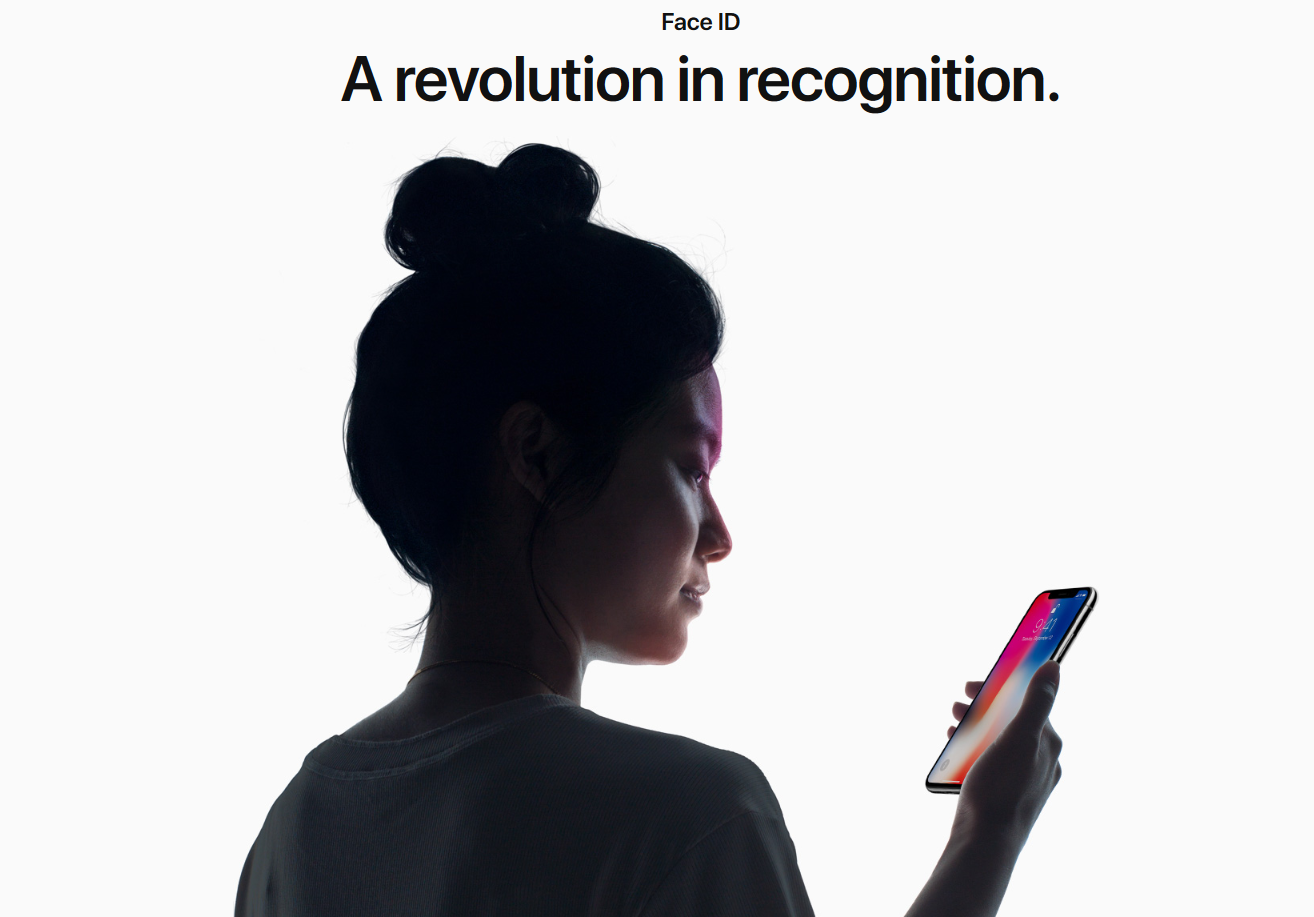
\includegraphics[width=1.0\textwidth]{figs/iphonex.png}
%\end{figure}
%\end{frame}
%
%\begin{frame}{Classification example 1}
%\begin{figure}
%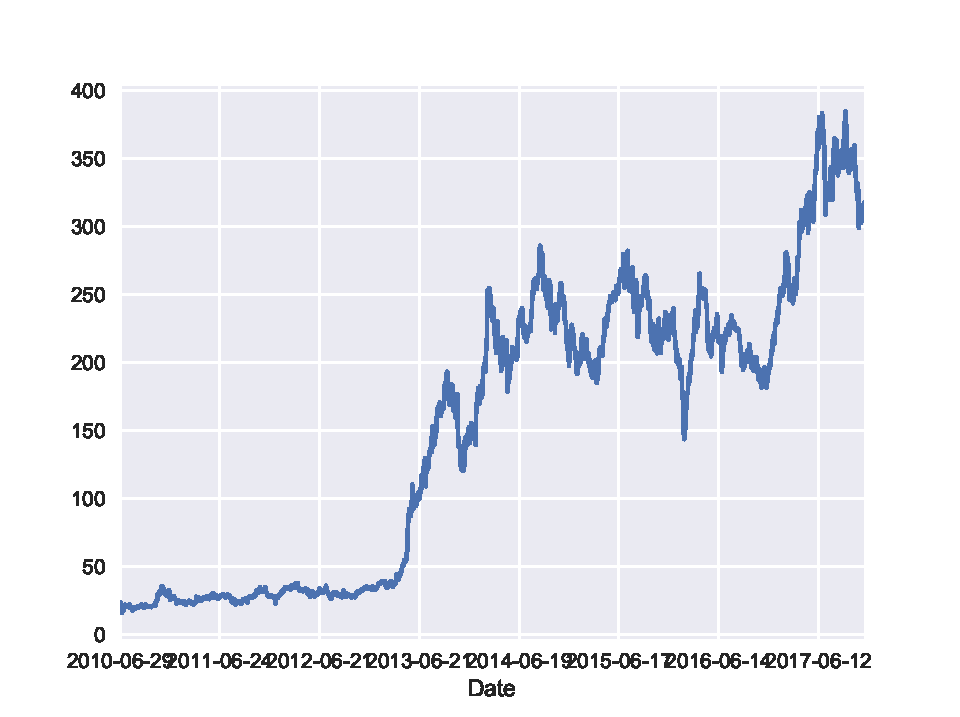
\includegraphics[width=1.0\textwidth]{figs/1.pdf}
%\end{figure}
%\end{frame}
%
%\begin{frame}{Classification example 2}
%\begin{figure}
%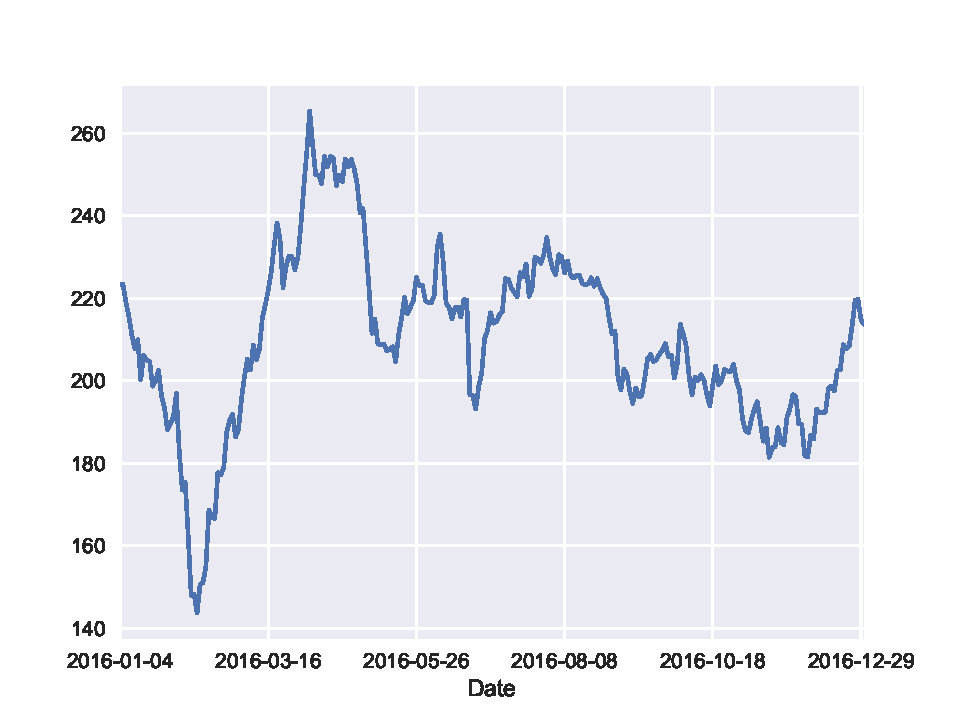
\includegraphics[width=1.0\textwidth]{figs/2.pdf}
%\end{figure}
%\end{frame}
%
%\begin{frame}{Classification example 3}
%\begin{figure}
%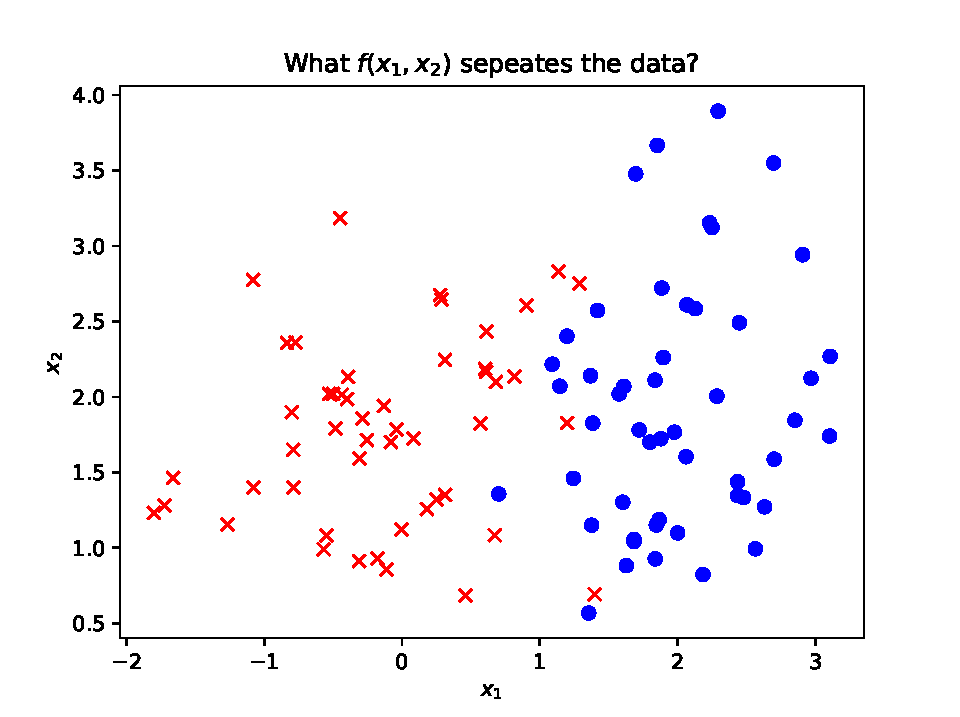
\includegraphics[width=1.0\textwidth]{figs/3.pdf}
%\end{figure}
%\end{frame}
%
%\begin{frame}{What is regression? }
%\begin{itemize}
%\item Can we find the trend in data?
%\item Can we predict the values in-between data points? 
%\item Classification is used everywhere!
%\item Ex: You are applying for a loan. The bank knows your income, job stability, and debt. How much of a loan can you get approved for?
%\item Variables: income, job stability, debt
%\item Output: How much \$ you get?
%\end{itemize}
%\end{frame}
%
%\begin{frame}{Linear regression: fitting a line to data}
%\begin{figure}
%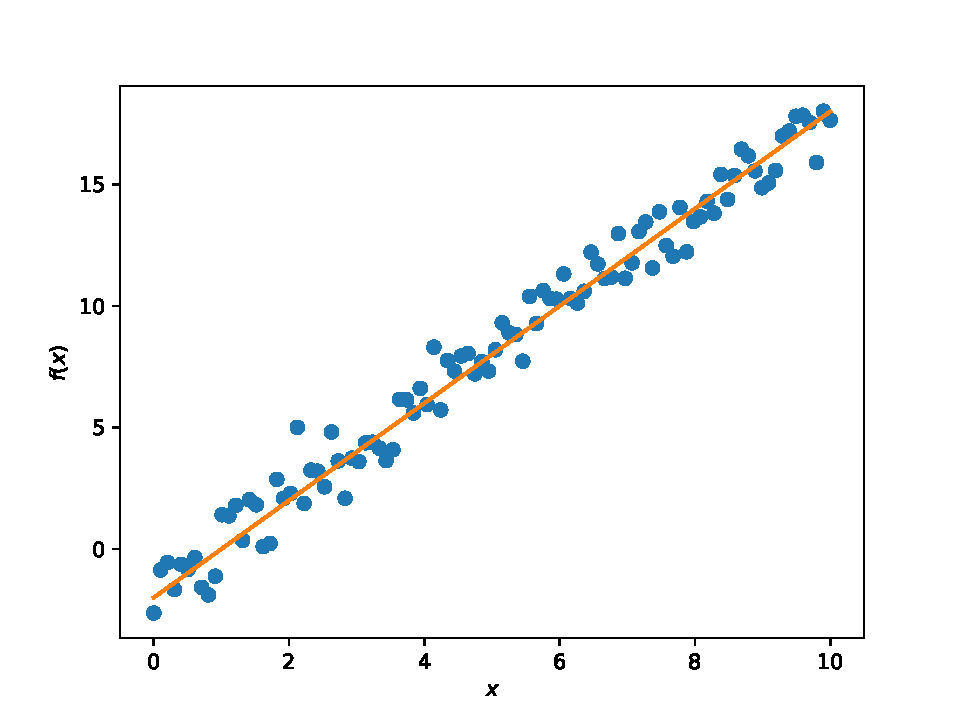
\includegraphics[width=1.0\textwidth]{figs/linear_regression.pdf}
%\end{figure}
%\end{frame}
%
%\begin{frame}{Kriging: using correlation between data}
%\begin{figure}
%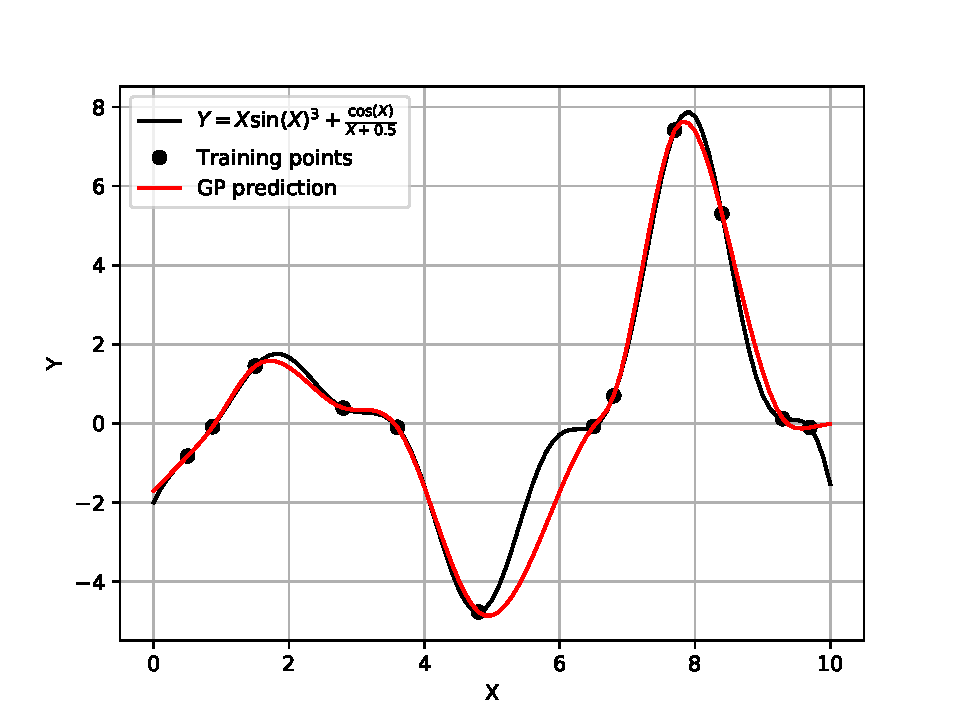
\includegraphics[width=1.0\textwidth]{figs/Kriging.pdf}
%\end{figure}
%\end{frame}
%
%\begin{frame}{What is clustering? Unsupervised learning}
%\begin{itemize}
%\item Can we find the structure in data?
%\item Can we detect and identify groups in data?
%\item Ex: We have a bunch of data related to income, job stability, and debt. Can we identify a pattern in the data?
%\item The key is that we don't know the label or value. 
%\item Ex: Used to identify similarities in protein chains 
%\end{itemize}
%\end{frame}
%
%\begin{frame}{Clustering: Can we categorize this data?}
%\begin{figure}
%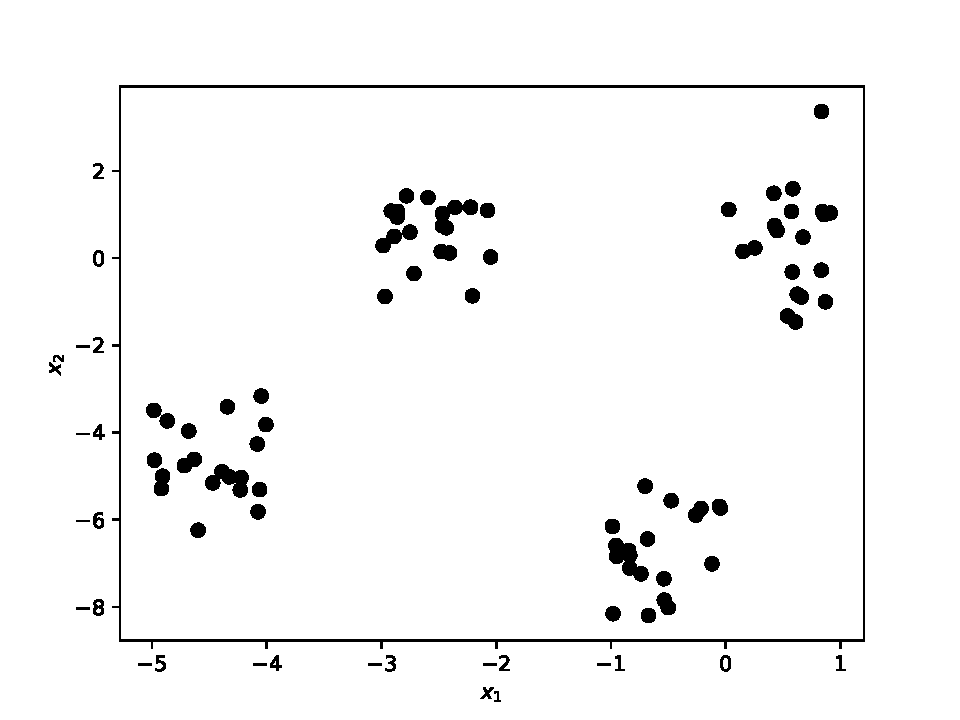
\includegraphics[width=1.0\textwidth]{figs/clust.pdf}
%\end{figure}
%\end{frame}
%
%\begin{frame}{Clustering output}
%\begin{figure}
%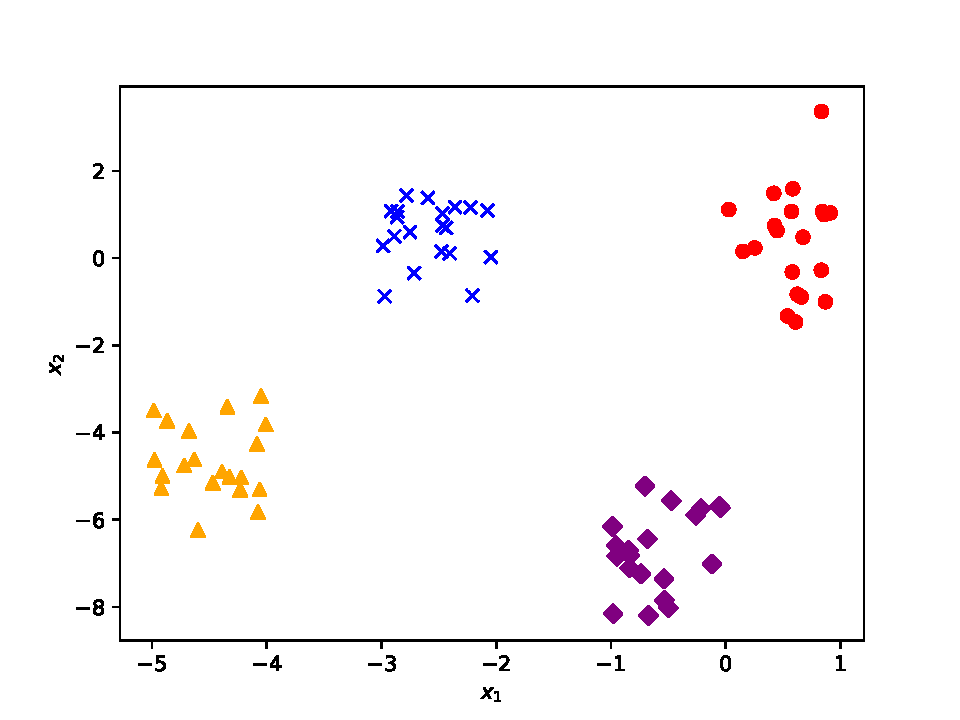
\includegraphics[width=1.0\textwidth]{figs/cluster.pdf}
%\end{figure}
%\end{frame}
%
%\begin{frame}{So what does the data look like for Scikit-Learn}
%Out input data will be a matrix (or numpy array) with $n$ number of samples and $d$ number of design variables (or \textbf{features})
%\begin{equation}
%\bm{X} = \begin{bmatrix}
%x_{11} & x_{12} & x_{13} & \cdots & x_{1d} \\ 
%x_{21} & x_{22} & x_{23} & \cdots & x_{2d} \\ 
%x_{31} & x_{32} & x_{33} & \cdots & x_{3d} \\ 
%\vdots & \vdots * \vdots & \vdots & \vdots \\
%x_{n1} & x_{n2} & x_{n3} & \cdots & x_{nd} \\ 
%\end{bmatrix}
%\end{equation}
%Each row of $\bm{X}$ represents a single sample.
%
%
%Out output data will be a vector $\bm{y}$ (usually a numpy array) with $n$ number samples.
%\begin{equation}
%\bm{y} = \begin{bmatrix}
%y_{1} \\
%y_{2} \\
%y_{3} \\
%\vdots \\
%y_{n} \\
%\end{bmatrix}
%\end{equation}
%\end{frame}
%
%\begin{frame}[fragile]{Let's consider a simple linear regression example}
%\begin{minted}
%{python}
%import numpy as np
%import matplotlib.pyplot as plt
%
%# let's create some arbitrary data
%# and fit a line to it
%
%np.random.seed(33)
%x = 10.0*np.random.random(100)
%noise = np.random.normal(loc=0.5, size=100)
%y = 2.3*x - 3 + noise
%plt.figure()
%plt.plot(X,y, 'o')
%plt.show()
%\end{minted}
%\end{frame}
%
%\begin{frame}[fragile]{Building a linear regression model}
%\begin{minted}
%{python}
%from sklearn.linear_model import LinearRegression
%# LinearRegression is a Python class that we'll use to create
%# our linear model object
%
%# we can't pass a vector into scikit-learn
%# instead we need to pass a feature matrix
%# we can do this by reshaping x
%X = x.reshape(-1,1)
%
%# we initialize a model object from the LinearRegression class
%# to begin the process. With the initialization, we can pass
%# model hyper-parameters, in this case we pass that a 
%# y intercept be determined
%model = LinearRegression(fit_intercept=True)
%\end{minted}
%\end{frame}
%
%\begin{frame}[fragile]{Fitting the linear regression model}
%\begin{minted}
%{python}
%# simply pass your training data into the model's fit function
%# which will run an 'optimization' selecting the best parameters
%# == this is the same as an ordinary least squares fit ==
%model.fit(X,y)
%
%# in this case there are two parameters for the line 
%# y = mx + b
%print('m = ', model.coef_)
%print('b = ', model.intercept_)
%# score calculates the R^2 (Coefficient of determination) 
%# for a given input and output 
%my_score = model.score(X,y)
%
%print('R^2 = ', my_score)
%\end{minted}
%\end{frame}
%
%\begin{frame}[fragile]{Predicting for new $x$ values}
%\begin{minted}
%{python}
%# let's generate new x values from slightly smaller than min(x)
%# to the slightly larger than the max(x)
%x_hat = np.linspace(np.min(x)-1.0,  np.max(x)+1.0, 100)
%
%# Again x_hat is a vector, and must be reshaped 
%# to be a 2 dimensional array
%X_hat = x_hat.reshape(-1, 1)
%
%# we can find new y_hat values by using the model.predict function
%y_hat = model.predict(X_hat)
%
%# let's plot the results
%plt.figure()
%plt.plot(X,y, 'o')
%plt.plot(x_hat, y_hat, '-')
%plt.show()
%\end{minted}
%\end{frame}
%
%\begin{frame}[fragile]{What about polynomials?}
%So let's consider a toy polynomial problem where
%\begin{equation}
%y = \beta_0 + \beta_1 x + \beta_2 x^2
%\end{equation}
%on the domain $-10.0 \leq x \leq 10.0$
%
%\begin{minted}
%{python}
%# generate artificial data
%np.random.seed(19)
%x = (10.0 + 10.0)* np.random.random(100) - 10.0
%noise = np.random.normal(scale=5.0,size=100)
%y = -1.0 + 2.2*x - 0.5*x**2 + noise
%
%plt.figure()
%plt.plot(x,y, 'o')
%plt.show()
%\end{minted}
%\end{frame}
%
%\begin{frame}[fragile]{Scikit-Learn includes a polynomial prepossessing tool}
%So in order the least squares regression, we need to construct the regression matrix $\bm{X}$. Scikit-Learn includes a Polynomial class for doing this easily.
%\begin{minted}
%{python}
%from sklearn.preprocessing import PolynomialFeatures
%# again we need to transfer x to a matrix... 
%# the reason is that sklearn doesn't deal with 1D data...
%X = x.reshape(-1,1)
%
%# create a poly object from the PolynomialFeatures class
%# in our case we'll be fitting a second order polynomial
%poly = PolynomialFeatures(degree=2)
%
%# now we use poly to transform our X into a Regression matrix!
%X = poly.fit_transform(X)
%print(X)
%# note this transformation includes the y intercept!
%\end{minted}
%\end{frame}
%
%\begin{frame}[fragile]{Fitting the second order polynomial}
%\begin{minted}
%{python}
%# create quad object from linear regression
%# the default is that fit_intercept = False
%# we don't want fit_intercept because it's included in X
%quad = LinearRegression(fit_intercept=False)
%
%# perform the least squares fit
%quad.fit(X,y)
%
%# predict for new values of x
%x_hat = np.linspace(np.min(x), np.max(x), 100)
%x_hat = x_hat.reshape(-1,1)
%X_hat = poly.fit_transform(x_hat)
%y_hat = quad.predict(X_hat)
%
%# plot the results
%plt.figure()
%plt.plot(x,y, 'o')
%plt.plot(x_hat, y_hat, '-')
%plt.show()
%\end{minted}
%\end{frame}
%
%\begin{frame}[fragile]{What are the resulting parameters?}
%Recall \begin{equation}
%y = \beta_0 + \beta_1 x + \beta_2 x^2
%\end{equation}
%
%You $\beta$ parameters are stored in the quad object.
%\begin{minted}
%{python}
%print('beta0 =', quad.coef_[0])
%print('beta1 =', quad.coef_[1])
%print('beta2 =', quad.coef_[2])
%\end{minted}
%\end{frame}
%
%\begin{frame}[fragile]{What about polynomials for higher dimensions?}
%Consider a polynomial response surface\begin{equation}
%f(x_1,x_2) = \beta_0 + \beta_1 x_1 + \beta_2x_2 + \beta_3x_1^2 + \beta_4x_1x_2 + \beta_5x_2^2
%\end{equation}
%\begin{minted}
%{python}
%# let's generate a 2 dimensional polynomial problem
%np.random.seed(121)
%X = np.random.random((100,2))
%# since this is a matrix, there is no need to reshape
%y = 1.0 + X[:,0] + 0.9*X[:,1] + 1.2*X[:,0]**2  \
%-1.3*X[:,0]*X[:,1] - 3.0*X[:,1]**2
%# plot the data
%from mpl_toolkits.mplot3d import Axes3D
%import matplotlib.pyplot as plt
%fig = plt.figure()
%ax = fig.add_subplot(111, projection='3d')
%ax.scatter(X[:,0], X[:,1], y, 'o')
%ax.set(xlabel='$x_1$', ylabel='$x_2$', zlabel='$f(x_1,x_2$')
%fig.show()
%\end{minted}
%\end{frame}
%
%\begin{frame}[fragile]{Same process for creating regression matrix and fitting}
%\begin{minted}
%{python}
%from sklearn.preprocessing import PolynomialFeatures
%poly = PolynomialFeatures(degree=2)
%X_train = poly.fit_transform(X)
%
%
%# fit the model
%model = LinearRegression(fit_intercept=False)
%model.fit(X_train,y)
%# print the model coefficients - you'll see they are exact!
%print(model.coef_)
%
%# Let's generate sampeles to predict over the domain
%x = np.linspace(np.min(X), np.max(X), 10)
%x1,x2 = np.meshgrid(x,x)
%X_hat = np.zeros((100,2))
%X_hat[:,0] = x1.flatten()
%X_hat[:,1] = x2.flatten()
%\end{minted}
%\end{frame}
%
%\begin{frame}[fragile]{Predicting and comparing the result}
%\begin{minted}
%{python}
%X_test = poly.fit_transform(X_hat)
%
%# predict for X_test
%Y_hat = model.predict(X_test)
%
%# reshape y_hat
%y_hat = Y_hat.reshape((10,10))
%
%# plot the results
%fig = plt.figure()
%ax = fig.add_subplot(111, projection='3d')
%ax.plot_surface(x1, x2, y_hat)
%ax.scatter(X[:,0], X[:,1], y, 'o', color='black')
%ax.set(xlabel='$x_1$', ylabel='$x_2$', zlabel='$f(x_1,x_2$')
%fig.show()
%\end{minted}
%\end{frame}
%
%\begin{frame}[fragile]{Classifcation with the famous flower database...}
%Naive Bayes Classification of Iris dataset...
%\begin{minted}
%{python}
%import seaborn as sns
%iris = sns.load_dataset('iris')
%
%X_iris = iris.drop('species', axis=1)
%y_iris = iris['species']  
%
%# sklearn includes tools for validation and model selection
%from sklearn.cross_validation import train_test_split
%Xtrain, Xtest, ytrain, ytest = train_test_split(X_iris, y_iris, random_state=1)   
%# this code splits the entire dataset into two
%# a training set and a testing set
%\end{minted}
%
%\end{frame}
%
%\begin{frame}[fragile]{The process for fitting models is same: apply NB}
%\begin{minted}
%{python}
%# 1. choose model class
%from sklearn.naive_bayes import GaussianNB 
%
%# 2. instantiate model
%model = GaussianNB()  
%   
%# 3. fit model to data                  
%model.fit(Xtrain, ytrain)   
%
%# 4. predict on new data                
%y_hat = model.predict(Xtest)
%
%# 5. score the model
%print(model.score(Xtest,ytest))          
%\end{minted}
%\end{frame}



\end{document}
